\subsection{Randomly Generated Colors}\label{ssec:colors}

In this example, we randomly generate $n=10^5$ colors using RGB values from 0 to 255,
and apply the SOM algorithm to illustrate how the sample points are organized.
We run the algorithm in batch mode (see Section~\ref{ssec:optimization}) with 500 total iterations, 
default learning-rate $\alpha(t)$ that decreases linearly from 0.05 to 0.01 per iteration,
and a hexagonal grid size $25 \times 25$ with toroidal boundaries. 
We use the Gaussian neighborhood function since it results in a smoother 
update to the codebook vectors.

\begin{figure}[t]
    \centering
    \begin{subfigure}[b]{0.4\textwidth}
        \centering
        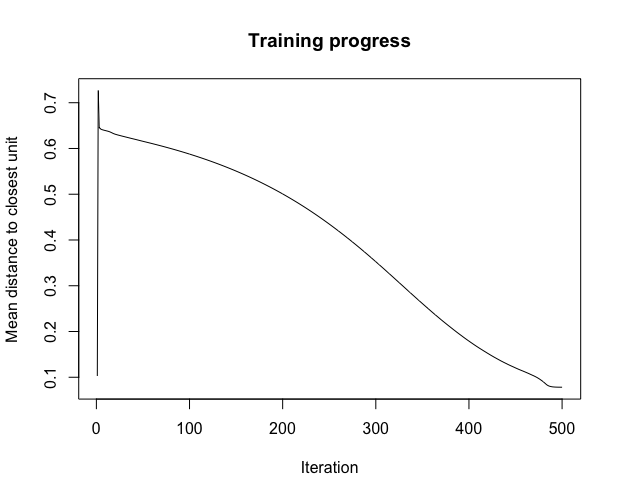
\includegraphics[width=\textwidth]{../figs/Colors-Gaussian-1.png}
        \caption{}
        \label{fig:colors-gauss-training}
    \end{subfigure}
    \begin{subfigure}[b]{0.4\textwidth}
        \centering
        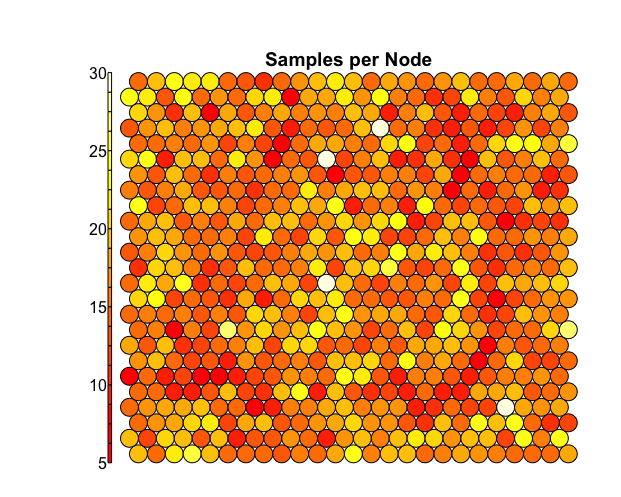
\includegraphics[width=\textwidth]{../figs/Colors-Gaussian-2.png}
        \caption{}
        \label{fig:colors-gauss-nodesize}
    \end{subfigure}
\end{figure}

Figure~\ref{fig:colors-gauss-training} shows that the algorithm 
seemed to converge as we see a slower decline in the mean distance to the closest unit.
Figure~\ref{fig:colors-gauss-nodesize} shows the number of samples assigned to each node
and we conclude that the grid size is reasonable since there are about 10-20
samples per node, which adheres to the general rule of thumb used by practitioners.

\begin{figure}[t]
    \centering
    \begin{subfigure}[b]{0.4\textwidth}
        \centering
        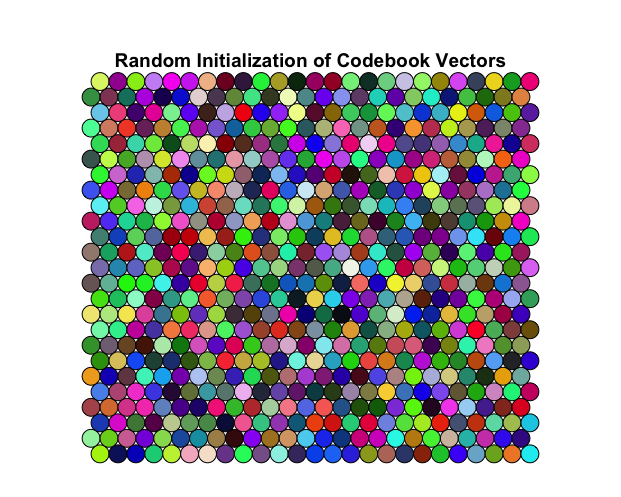
\includegraphics[width=\textwidth]{../figs/Colors-Bubble-5.png}
        \caption{}
        \label{sfig:color-random}
    \end{subfigure}
    \begin{subfigure}[b]{0.4\textwidth}
        \centering
        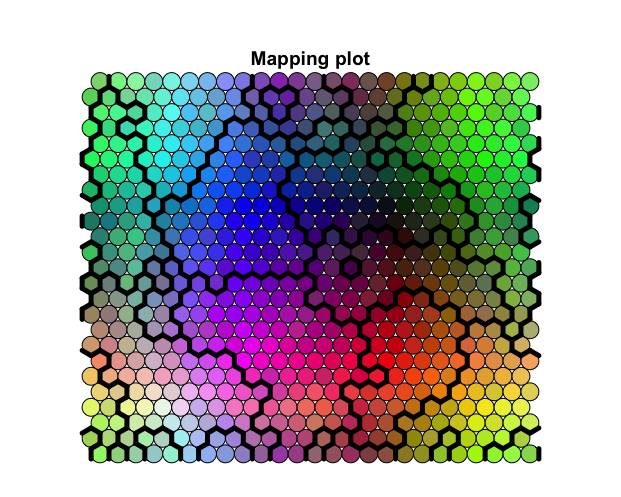
\includegraphics[width=\textwidth]{../figs/Colors-Gaussian-6.png}
        \caption{}
        \label{sfig:color-gauss-code}
    \end{subfigure}
    \caption{Figure~\ref{sfig:color-random} visualizes 
        a random initialization of the codebook vectors.
        Figure~\ref{sfig:color-gauss-code}
        visualizes the trained codebook vectors for SOM with 
        the Gaussian neighborhood function and cluster boundaries
        defined by hierarchical clustering.}
    \label{fig:colors-codebook}
\end{figure}

Figure~\ref{fig:colors-codebook} shows the color representations of the codebook vectors. 
Qualitatively, the algorithm seems to have successfully ``ordered'' the data
as the color spectrum smoothly transitions throughout the nodes.
In this particular example, we can easily interpret this output.
The nodes became detectors of certain types of colors,
e.g.\ the red nodes are trained to detect red-like color inputs, 
the green nodes are trained to detect green-like color inputs, etc.

\begin{figure}[t]
    \centering
    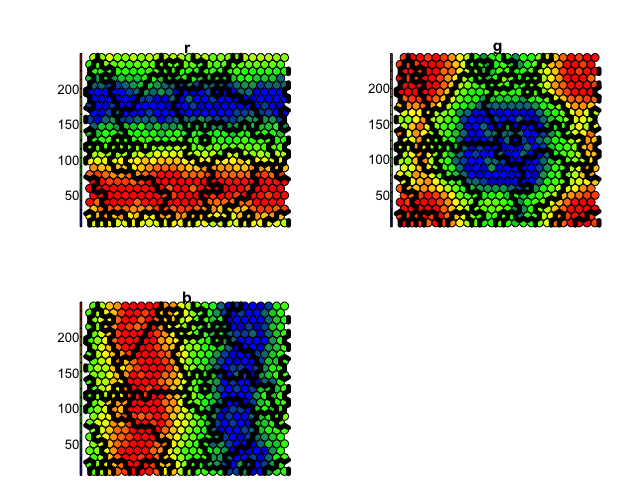
\includegraphics[width=\textwidth]{../figs/Colors-Gaussian-8.png}
    \caption{}
    \label{fig:colors-gauss-feature}
    \caption{Plot of each component of trained codebook vectors for SOM using the Gaussian
            neighborhood function.}
\end{figure}

In Figure~\ref{fig:colors-gauss-feature},
we plot the codebook vectors for each component (hence, each feature).
The color spectrum ranges from blue to green to red in increasing order. 
Note that there is a component changing horizontally (red)
one component changing vertically (blue),
and one component changing radially (green).
The three features are exchangeable 
since each component is uniformly and independently sampled,
so there is no significant relationship between the components and their exhibited behavior.
This seems to suggest that all three components add independent information
to the structure of the data, which is reasonable since the three color components are independent quantities.
While it is unclear exactly why we see this strong horizontal, vertical, and radial pattern,
other experiments show that the codebook vectors tend to attain values 
that are ordered along the axes of the network~\cite{kohonen:1990}.
